

\begin{table*}
    \centering
    \large
    \begin{tabular}{l P{0.08\textwidth}P{0.08\textwidth} P{0.08\textwidth}P{0.08\textwidth}  P{0.08\textwidth}P{0.08\textwidth}}
        \mr{2}{Métrica}          &\multicolumn{2}{c}{Sin Contexto}& \multicolumn{2}{c}{Tweet}          &  \multicolumn{2}{c}{Tweet + Cuerpo}    \\
                  & $\neg$FT &  FT     & $\neg$FT&    FT       &$\neg$FT &    FT \\
        \hline
        Accuracy  & $88.9$   &  $89.9$ & $90.2$  &$\mbf{91.0}$ & $90.4$  &  $90.5$ \\
        Precisión & $67.8$   &  $71.8$ & $73.1$  &$\mbf{74.8}$ & $73.9$  &  $72.8$ \\
        Recall    & $56.8$   &  $60.2$ & $60.1$  &$\mbf{65.3}$ & $61.1$  &  $64.1$ \\
        F1        & $61.8$   &  $65.5$ & $66.0$  &$\mbf{69.7}$ & $66.9$  &  $68.1$ \\
        Macro  F1 & $77.6$   &  $79.8$ & $80.1$  &$\mbf{82.2}$ & $80.6$  &  $81.3$ \\
        \hline
    \end{tabular}


    \caption{Resultados de los experimentos de clasificación para la tarea \emph{binaria} de detección de discurso de odio, expresados como la media de las distintas métricas sobre diez corridas independientes. En negrita, los mejores resultados. Cada modelo es un BERT con tres posibles entradas: sólo el comentario (\emph{Sin contexto}), el tweet de la noticia a la cual responde el comentario (\emph{Tweet}), y el tweet más el cuerpo de la noticia (\emph{Tweet + Cuerpo}). Para cada una de estas posibilidades usamos dos versiones: una sobre BETO ($\neg$FT) y otra sobre BETO ajustado al dominio (FT).}
    \label{tab:task_a_results}
\end{table*}


La Tabla \ref{tab:task_a_results} contiene los resultados para la tarea de clasificación \tbf{binaria} medidos por Accuracy, Precision, Recall, F1 de la clase positiva y Macro F1 entre las dos clases. Las métricas están expresadas como las medias de diez corridas independientes de los experimentos. Las seis columnas corresponden a la combinación de los tres posibles modelos dependiendo del contexto utilizado y de acuerdo a si ajustamos al dominio o no. Podemos observar que, en todos los casos, la adaptación de dominio (las columnas marcadas con FT) obtienen mejor rendimiento que los modelos que no están adaptados ($\neg$FT) resultando en una mejora de alrededor de 4 puntos de F1 en los casos sin contexto y con contexto de tweet. Entre los modelos sin ajustar a dominio, el que consume el contexto completo (tweet + cuerpo de la noticia) obtiene el mejor desempeño; sin embargo, esto no se replica en el caso ajustado a dominio, donde gana el contexto simple. Viendo sólo las columnas marcadas como $FT$, la mejora contra el modelo que no consume contexto es de $4.2$ puntos de F1. El modelo con el contexto completo, si bien mejora la performance general contra no tener contexto, pierde precisión al ser adaptado al dominio.


\begin{table*}
    \centering
    \Large
    \begin{tabular}{l P{0.08\textwidth}P{0.08\textwidth} P{0.08\textwidth}P{0.08\textwidth}  P{0.08\textwidth}P{0.08\textwidth}}
        Métrica        &\mc{2}{Sin Contexto}& \mc{2}{Tweet}          &  \mc{2}{Tweet + Cuerpo}    \\
                       & $\neg$FT&    FT    & $\neg$FT   &    FT     & $\neg$ FT&    FT     \\
        \hline
        LLAMA          & $64.6$ &    $65.1$   & $63.8$ &$\mbf{68.5}$  & $65.3$ &    $68.0$    \\
        MUJER          & $37.3$ &    $38.9$   & $41.1$ &$\mbf{42.1}$  & $38.1$ &$\mbf{42.1}$ \\
        LGBTI          & $35.1$ &    $36.6$   & $45.1$ &$\mbf{48.2}$  & $42.7$ &    $44.5$    \\
        RACISMO        & $63.5$ &    $65.3$   & $68.8$ &$\mbf{72.0}$  & $69.1$ &    $71.1$    \\
        CLASE          & $40.1$ &    $43.3$   & $49.1$ &$\mbf{51.1}$  & $45.1$ &    $47.6$    \\
        POLITICA       & $55.5$ &    $61.1$   & $57.9$ &$62.5$        & $59.1$ &$\mbf{64.8}$ \\
        DISCAPAC       & $55.1$ &    $58.2$   & $58.5$ &$\mbf{60.9}$  & $55.7$ &    $57.8$    \\
        APARIENCIA     & $72.6$ &    $74.2$   & $74.1$ &$\mbf{76.6}$  & $75.5$ &    $75.8$    \\
        CRIMINAL       & $51.3$ &    $52.9$   & $65.0$ &$\mbf{69.9}$  & $65.4$ &    $66.8$    \\
        \hline
        Macro F1       & $52.8$ &    $55.1$   & $58.2$ &$\mbf{0.613}$ & $57.3$ &    $59.8$    \\
        Macro Precision& $55.8$ &    $63.0$   & $64.2$ &$\mbf{0.702}$ & $67.7$ &    $67.8$    \\
        Macro Recall   & $50.6$ &    $49.9$   & $54.0$ &$\mbf{0.551}$ & $50.4$ &    $54.1$    \\
        % \hline
        % Hate Precision & 0.679 &    0.712   & 0.722 &\textbf{0.760}  & 0.748 &    0.741    \\
        % Hate Recall    & 0.621 &    0.631   & 0.642 &\textbf{0.666}  & 0.621 &    0.658    \\
        % Hate F1        & 0.648 &    0.668   & 0.679 &\textbf{0.710}  & 0.679 &    0.697    \\
        \bottomrule
        \end{tabular}
    \caption{Resultados de los experimentos de clasificación para la tarea \emph{granular} de detección de discurso de odio, expresados como la media de las distintas métricas sobre diez corridas independientes. Cada modelo es un BERT con tres posibles entradas: sólo el comentario (\emph{Sin contexto}), el tweet de la noticia a la cual responde el comentario (\emph{Tweet}), y el tweet más el cuerpo de la noticia (\emph{Tweet + Cuerpo}). Para cada una de estas posibilidades usamos dos versiones: una sobre BETO($\neg$FT) y otra sobre BETO ajustado al dominio (FT) de acuerdo a lo descripto en la Sección \ref{sec:contextualized_classifiers}}
    \label{tab:task_b_results}
\end{table*}



La Tabla \ref{tab:task_b_results} muestra los resultados de los experimentos de clasificación para la tarea de detección \tbf{granular} medidos en puntos de F1 para cada una de las características, y las métricas promediadas de precision, recall, y F1. Como era esperable, la ganancia de tener contexto disponible es más evidente en esta tarea, observándose una diferencia de aproximadamente 6 puntos de F1 entre la mejor versión sin contexto y la mejor versión con contexto ($55.1$ Macro F1 de la versión $FT$ sin contexto vs $61.3$ F1 de la versión $FT$ con el contexto del tweet). Respecto a los dos tipos de contexto, de nuevo la versión simple obtiene mejor rendimiento en prácticamente todas las características, con la única excepción de POLITICA.


\begin{figure*}[]
    \centering
    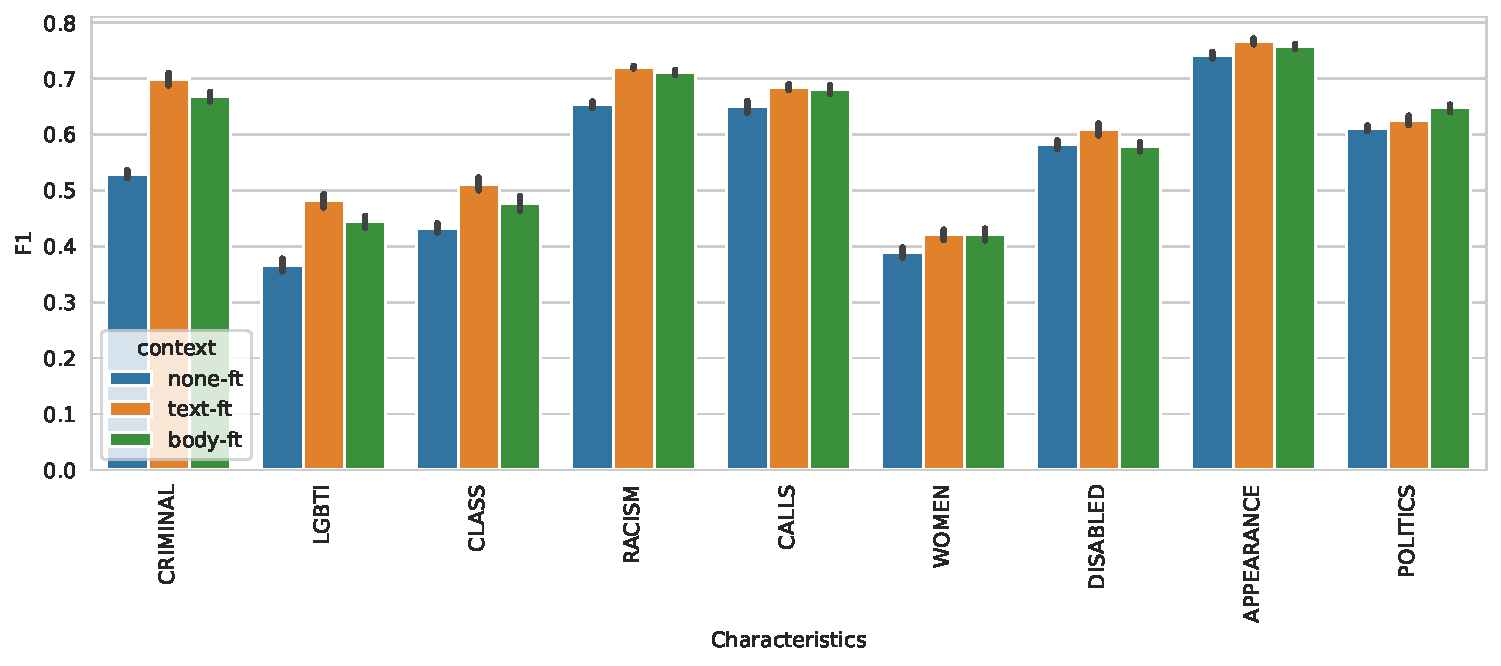
\includegraphics[width=\textwidth]{img/task_b_scores.pdf}
    \caption{Métrica F1 para cada característica de la tarea granular. Las características están ordenadas de mayor a menor de acuerdo a la diferencia de performance entre el modelo sin contexto y el modelo contextualizado. }
    \label{fig:barplot_task_b_results}
\end{figure*}

La Figura \ref{fig:barplot_task_b_results} muestra los resultados por característica ordenados de mayor a menor según la diferencia de rendimiento entre los clasificadores ajustados a dominio que consumen contexto y aquellos que no lo hacen. Para todas las características se observa una mejora estadísticamente significativa al correr un test Mann-Whitney U ($p \leq 0.005$, p valores ajustados por múltiples comparaciones con Benjamini-Hochberg \cite{benjamini1995controlling}). Las diferencias más sustanciales se dan en el caso de CRIMINAL ($+17$ puntos F1 de diferencia), LGBTI ($+12$ puntos), CLASE ($+8$ puntos), y RACISMO (casi $+7$). Del otro lado, las características con menos mejora son APARIENCIA y POLITICA, algo esperable dado que el fenómeno tiene características poco dependientes del contexto como observamos en algunos ejemplos de la Sección \ref{sec:analisis_dataset_por_caracteristica} y por la misma definición y ejemplos considerados (ver Apéndice \ref{app:05}). Finalmente, y como resumen de estas tablas, se observa que los modelos con contexto simple son los que mejor performance tienen, en general y para cada característica, con la excepción de POLITICA.


\begin{figure}[ht!]
    \centering
    \small
    \begin{subfigure}[b]{\textwidth}
        \centering
        \caption{Precisión}
        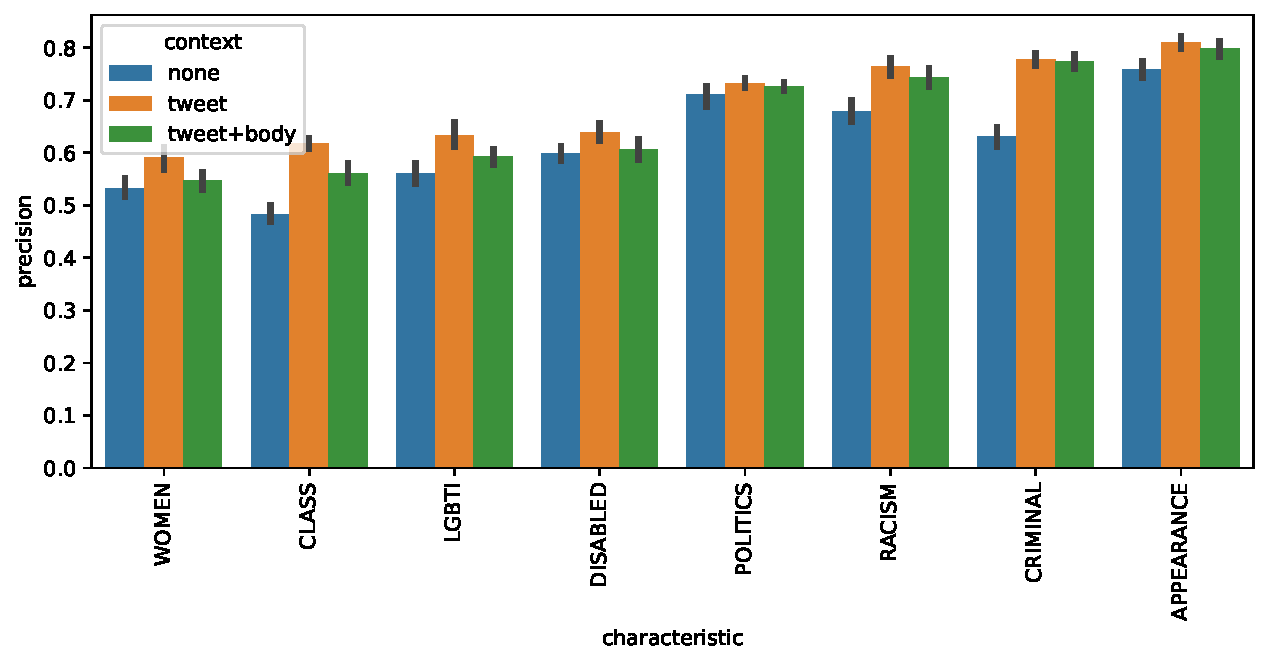
\includegraphics[width=0.75\textwidth]{img/06/precision_barplot.pdf}

    \end{subfigure}
    \begin{subfigure}[b]{\textwidth}
        \centering
        \caption{Sensibilidad exacta}
        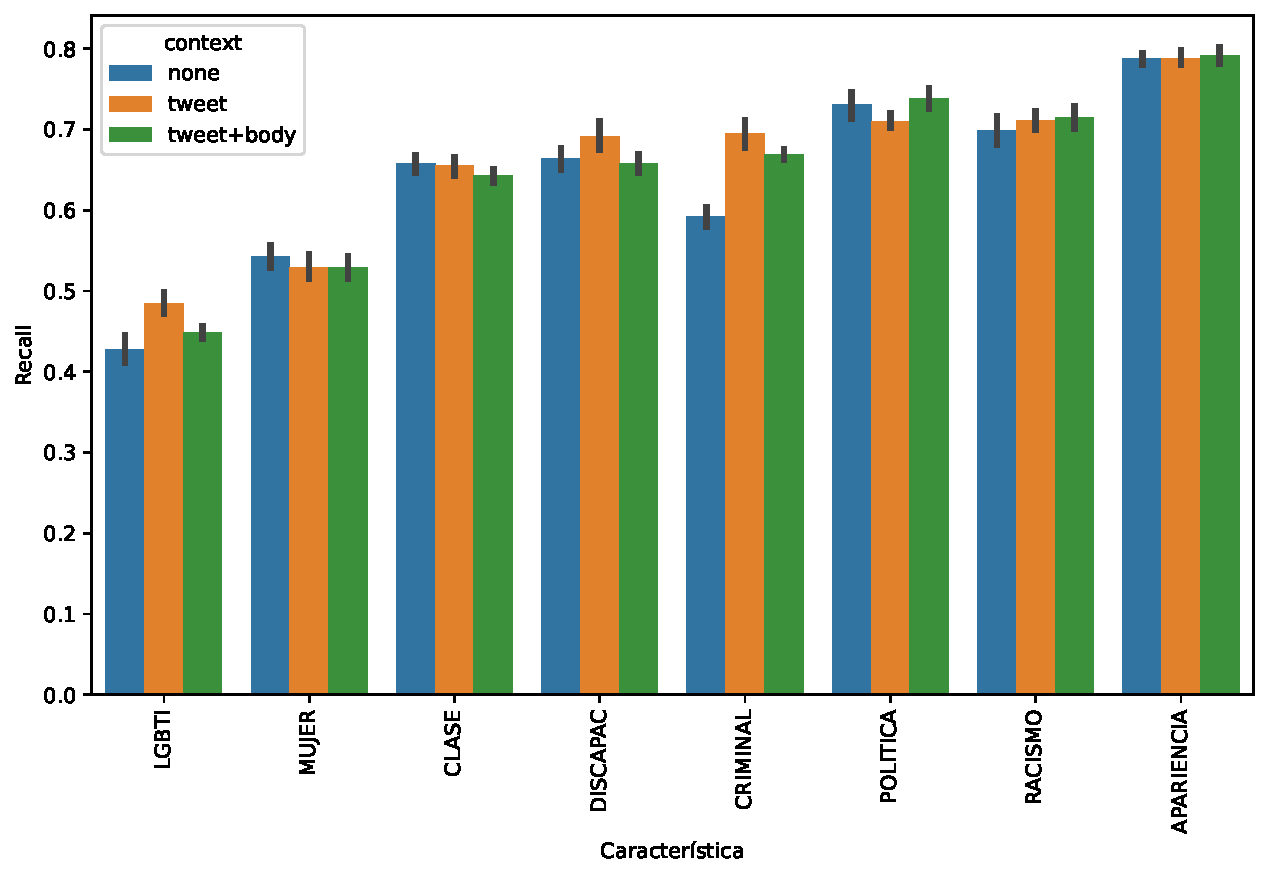
\includegraphics[width=0.75\textwidth]{img/06/exact_recall_barplot.pdf}

        \label{subfig:exact_recall}
    \end{subfigure}
    \begin{subfigure}[b]{\textwidth}
        \centering
        \caption{Sensibilidad total}
        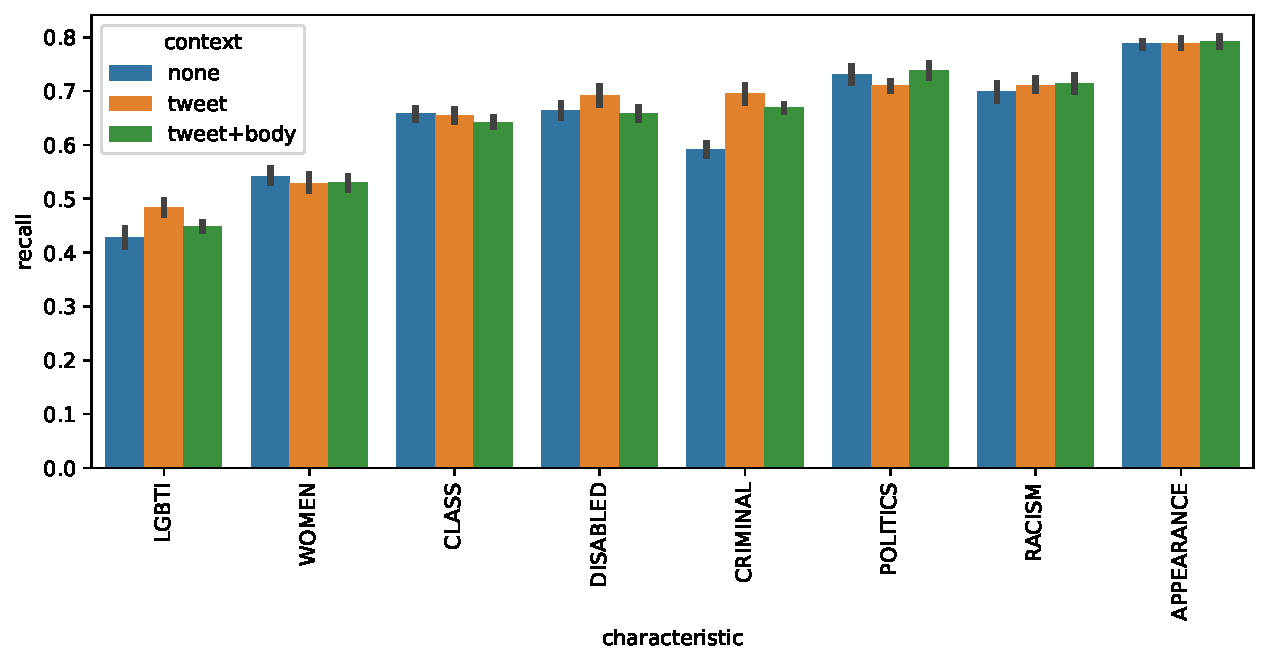
\includegraphics[width=0.75\textwidth]{img/06/hate_recall_barplot.pdf}

        \label{subfig:total_recall}
    \end{subfigure}
    \caption{Precisión y sensibilidad para cada característica de la tarea granular. Las diferentes barras marcan el tipo de contexto que recibe el clasificador. Sensibilidad exacta (Figura \ref{subfig:exact_recall}) cuenta la sensibilidad sobre la salida exacta de cada categoría, mientras que la sensibilidad total cuenta como recuperado un tweet si al menos alguna característica del clasificador lo marca como discurso de odio.}
    \label{fig:precision_recall_granular_classifier}
\end{figure}

Una forma distinta de evaluar el rendimiento de los clasificadores granulares es de acuerdo a su sensibilidad o capacidad de recuperación de comentarios discriminatorios, aún cuando esto ocurra por el motivo incorrecto. La Figura \ref{fig:precision_recall} ilustra esta comparación analizando la sensibilidad de dos maneras: exacta, donde consideramos recuperado un tweet sólo si el clasificador acierta a la característica analizada (es decir, si la característica es MUJER, el clasificador debe predecir MUJER); y total, donde consideramos un tweet recuperado si alguna característica es marcada por el clasificador independientemente de si es la correcta. Podemos ver que la categoría MUJER pasa de ser la de menor sensibilidad a dejar a la categoría LGBTI como la que tiene menor tasa de comentarios ofensivos recuperados. Análogamente, la categoría CLASE obtiene una mejora sustancial en su sensibilidad, algo compatible con el hecho de su solapamiento con otras características como RACISMO, POLITICA y CRIMINAL observado en la Figura \ref{fig:heatmap_characteristics}. También puede observarse que, en líneas generales, el contexto favorece una mejora de la precisión para cada característica y también un mayor recall exacto. Para el caso de la sensibilidad total, el desempeño de los clasificadores se empareja entre las versiones contextualizadas y no contextualizadas para cada característica con la excepción notoria de LGBTI y CRIMINAL.

\begin{table}[hb!]
    \centering
    \begin{tabular}{l P{0.10\textwidth}P{0.10\textwidth} P{0.10\textwidth}P{0.10\textwidth}  P{0.10\textwidth}P{0.10\textwidth}}
                  &\mc{2}{Sin Contexto}& \mc{2}{Tweet}          &  \mc{2}{Tweet + Cuerpo}    \\
                  & Bin   &    Gran         & Bin   &    Gran     & Bin  &   Gran     \\
        \hline
        Precision &  $71.8$ &  $71.1$       &  $74.8$& $\mbf{75.9}$ & $72.8$ & $74.0$ \\
        Recall    &  $60.2$ &  $63.6$       &  $65.3$& $\mbf{66.7}$ & $64.1$ & $66.0$ \\
        F1        &  $65.5$ &  $67.1$       &  $69.7$& $\mbf{71.0}$ & $68.1$ & $69.7$ \\
        Macro F1  &  $79.8$ &  $80.6$       &  $82.2$& $\mbf{83.0}$ & $81.3$ & $82.2$ \\
        \hline
        \end{tabular}
    \caption{Desempeño de los modelos para la tarea de detección binaria de discurso de odio. Los modelos considerados son modelos \beto{} ajustados a dominio que consumen tres tipos de entrada: sin contexto, tweet, y tweet+cuerpo. Dos posibles entrenamientos fueron evaluados: sobre la tarea binaria (\tbf{Bin}) o sobre la tarea granular (\tbf{Gran}).}
    \label{tab:plain_vs_granular_hate_detection}
\end{table}


Como se mencionó en la Sección \ref{sec:tasks}, un clasificador sobre la tarea granular puede convertirse fácilmente en uno para la tarea binaria tomando la disyunción lógica de sus salidas: si se detecta al menos una característica ofendida, entonces el tweet contiene discurso de odio. De esta forma, podemos evaluar el desempeño en la tarea binaria de aquellos clasificadores entrenados para la tarea granular. La Tabla \ref{tab:plain_vs_granular_hate_detection} muestra esta comparativa para las distintas métricas sobre los clasificadores ajustados a dominio. Podemos observar que, en todos los casos, entrenar el modelo sobre la tarea granular produce pequeñas mejoras en la performance de los clasificadores entrenados sobre la tarea binaria (aproximadamente $+0.8$ puntos de Macro F1 en cada de uno).

